\subsubsection{\stid{4.13} ECP/VTK-m}

\paragraph{Overview}
The ECP/VTK-m project is providing the core capabilities to perform scientific visualization on Exascale architectures.
The ECP/VTK-m project fills the critical feature gap of performing visualization and analysis on processors like graphics-based processors.
The results of this project will be delivered in tools like ParaView, VisIt, and Ascent as well as in stand-alone form.
Moreover, these projects are depending on this ECP effort to be able to make effective use of ECP architectures.

One of the biggest recent changes in high-performance computing is the increasing use of accelerators.
Accelerators contain processing cores that independently are inferior to a core in a typical CPU, but these cores are replicated and grouped such that their aggregate execution provides a very high computation rate at a much lower power.

Current and future CPU processors also require much more explicit parallelism.
Each successive version of the hardware packs more cores into each processor, and technologies like hyper threading and vector operations require even more parallel processing to leverage each core's full potential.

VTK-m is a toolkit of scientific visualization algorithms for emerging processor architectures.
VTK-m supports the fine-grained concurrency for data analysis and visualization algorithms required to drive extreme scale computing by providing abstract models for data and execution that can be applied to a variety of algorithms across many different processor architectures.

The ECP/VTK-m project is building up the VTK-m codebase with the necessary visualization algorithm implementations that run across the varied hardware platforms to be leveraged at the Exascale.
We will be working with other ECP projects, such as ALPINE, to integrate the new VTK-m code into production software to enable visualization on our HPC systems.

\paragraph{Key  Challenges}
The scientific visualization research community has been building scalable HPC algorithms for over 15 years, and today there are multiple production tools that provide excellent scalability.
However, our current visualization tools are based on a message-passing programming model.
More to the point, they rely on a coarse decomposition with ghost regions to isolate parallel execution \cite{Ahrens2001,Childs2010}.
However, this decomposition works best when each processing element has on the order of a hundred thousand to a million data cells \cite{ParaViewTutorial} and is known to break down as we approach the level of concurrency needed on modern accelerators \cite{Moreland2012:Ultravis,Moreland2013:UltraVis}.

DOE has made significant investments in HPC visualization capabilities.
For us to feasibly update this software for the upcoming Exascale machines, we need to be selective on what needs to be updated, and we need to maximize the code we can continue to use.
Regardless, there is a significant amount of software to be engineered and implemented, so we need to extend our development resources by simplifying algorithm implementation and providing performance portability across current and future devices.


\paragraph{Solution Strategy}
The ECP/VTK-m project leverages VTK-m \cite{Moreland2016:VTKm} to overcome these key challenges.
VTK-m has a software framework that provides the following critical features.

\begin{enumerate}
\item \textbf{Visualization building blocks:}
  VTK-m contains the common data structures and operations required for scientific visualization.
  This base framework simplifies the development of visualization algorithms \cite{VTKmUsersGuide}.
\item \textbf{Device portability:}
  VTK-m uses the notion of an abstract device adapter, which allows algorithms written once in VTK-m to run well on many computing architectures.
  The device adapter is constructed from a small but versatile set of data parallel primitives, which can be optimized for each platform \cite{Blelloch1990}.
  It has been shown that this approach not only simplifies parallel implementations, but also allows them to work well across many platforms \cite{Lo2012,Larsen2015,Moreland2015}.
\item \textbf{Flexible integration:}
  VTK-m is designed to integrate well with other software.
  This is achieved with flexible data models to capture the structure of applications' data \cite{Meredith2012} and array wrappers that can adapt to target memory layouts \cite{Moreland2012:PDAC}.
\end{enumerate}

Even with these features provided by VTK-m, we have a lot of work ahead of us to be ready for Exascale.
Our approach is to incrementally add features to VTK-m and expose them in tools like ParaView and VisIt.


\begin{figure}[t]
  \centering
  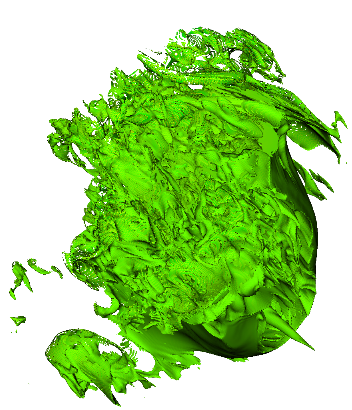
\includegraphics[height=1.5in]{projects/2.3.4-DataViz/2.3.4.13-ECP-VTK-m/VTKm-Clip}\quad
  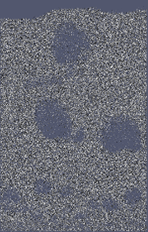
\includegraphics[height=1.5in]{projects/2.3.4-DataViz/2.3.4.13-ECP-VTK-m/VTKm-Bubbles-Density}
  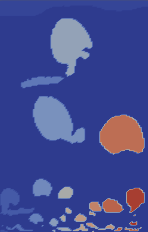
\includegraphics[height=1.5in]{projects/2.3.4-DataViz/2.3.4.13-ECP-VTK-m/VTKm-Bubbles-Components}\quad
  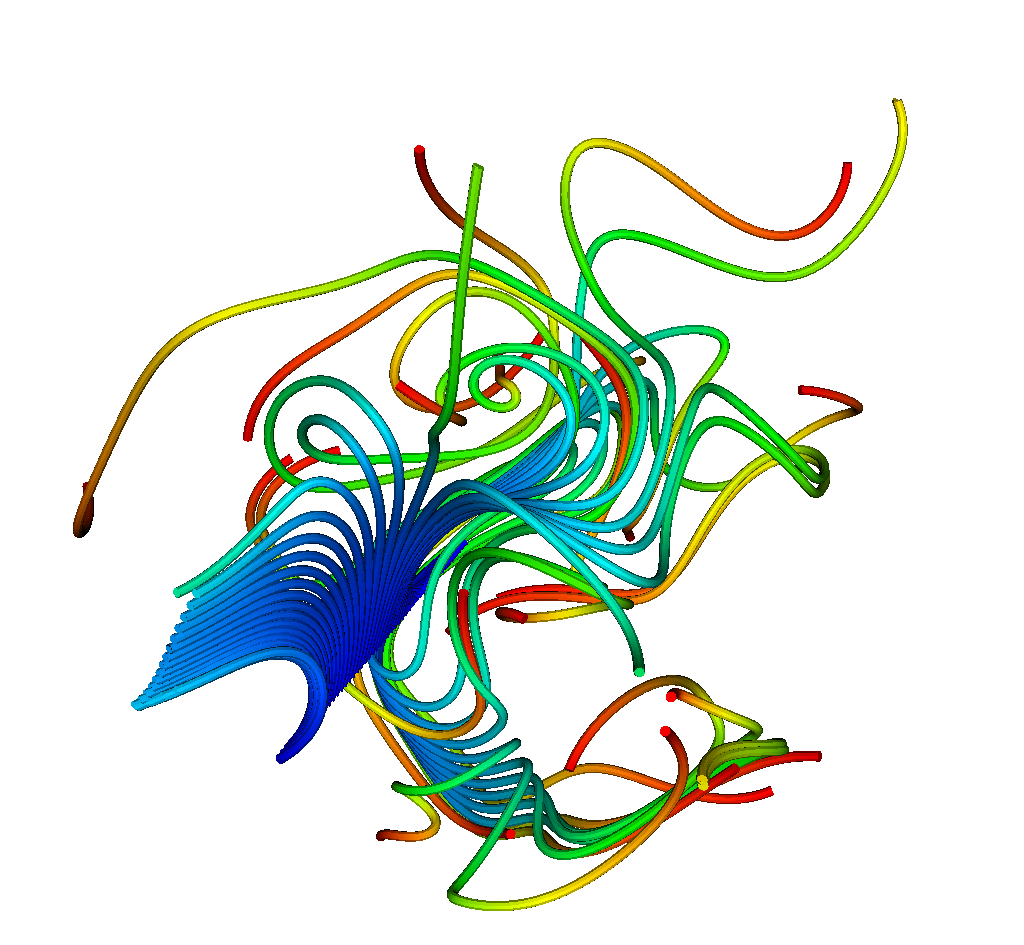
\includegraphics[height=1.5in]{projects/2.3.4-DataViz/2.3.4.13-ECP-VTK-m/VTKm-Streamlines}
  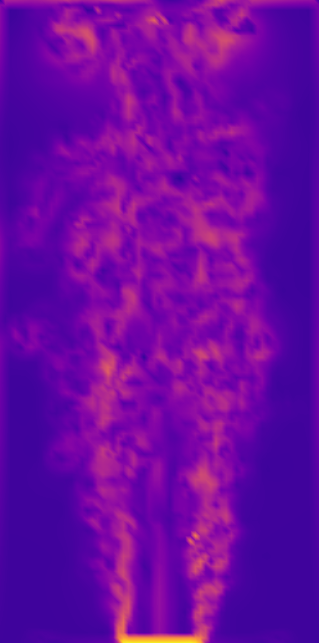
\includegraphics[height=1.5in]{projects/2.3.4-DataViz/2.3.4.13-ECP-VTK-m/VTKm-FTLE}
  \caption{
    Examples of recent progress in VTK-m include (from left to right) clipping to form an interval volume, connected components to identify bubbles of low density, advection of particles through time, and a generated FTLE field to identify Lagrangian coherent surfaces.
  }
  \label{fig:VTKmRecent}
\end{figure}

\paragraph{Recent Progress}
The VTK-m project is organized into many implementation activities.
The following features have been completed in the FY19 fiscal year.

\begin{itemize}
\item \textbf{VTK-m Releases:}
  VTK-m 1.3 was released in November 2018.
  VTK-m 1.4 was released in June 2019.
  VTK-m 1.5 was released in October 2019.
\item \textbf{ZFP}
  Working in collaboration with the ZFP project (now part of WBS 2.3.4.16), the ZFP compression algorithm \cite{zfp-jsm2017} is implemented in VTK-m.
  This implementation ports across ECP platforms.
\item \textbf{Clipping:}
  A common visualization operation for extracting regions of interest, clipping provides mesh cutaways and interval volumes as demonstrated in Figure \ref{fig:VTKmRecent}.
%% \item \textbf{Ghost Cells:}
%%   Provided support for defining and stripping ghost cell information.
\item \textbf{Merge Points:}
  It is often necessary to collect together positions in 3-space that are nearby \cite{Yenpure2019}.
\item \textbf{Connected Components:}
  It can be physically significant to identify groups of elements that are mutually connected by either topology or common field attributes as demonstrated in Figure \ref{fig:VTKmRecent}.
\item \textbf{Particle Advection:}
  Many flow visualization algorithms depend on computing the movement of weightless particles in a flow vector field, which may change over time \cite{Pugmire2018}.
  These include stream lines, path lines, Lagrangian coherent structures, and stream surfaces as demonstrated in Figure \ref{fig:VTKmRecent}.
  We have also added tube geometry to improve rendering representation.
%% \item \textbf{Mesh Warping:}
%%   Simulations often represent Lagrangian movements in terms of displacements, which have to be applied to geometry to be properly visualized.
%% \item \textbf{Contouring:}
%%   All 3D cell shapes are now supported in our contouring algorithm.
\item \textbf{Mesh Quality:}
  Cell metrics provide important physical and meta information about a geometry.
\item \textbf{Surface Normals:}
  Surface normals are an important feature for proper representation in rendering.
  Ensuring consistent ordering is important to avoid rendering artifacts.
\item \textbf{Lightweight Cell Library:}
  To help consolidate common code between VTK-m and other software, the code for cell management has been extracted into its own lightweight library.
%% \item \textbf{Extruded Cell Sets:}
%%   ECP's XGC simulation code uses an extrusion of a surface mesh for its data representation.
%%   A similar representation is added to VTK-m for zero-copy data ingestion.
\end{itemize}

\paragraph{Next Steps}
Our next efforts include:

\begin{itemize}
%% \item \textbf{Structured Grid Contouring:}
%%   There are several optimizations that can be made for contouring in structured grids.
\item \textbf{Performance Regression Testing:}
  It is important to ensure that in addition to being correct, the performance of VTK-m code does not regress.
\item \textbf{Kokkos Devices:}
  We will explore the feasibility of using the Kokkos libraries to implement the device porting layer.
%% \item \textbf{Improved Testing:}
%%   We plan to improve the testing layer by supporting image comparison and data files.
\item \textbf{Higher Order Meshes:}
  Many ECP simulations use high order interpolation techniques on their meshes.
\end{itemize}

\noindent
{\tiny Sandia National Laboratories is a multimission laboratory managed and operated by National Technology \& Engineering Solutions of Sandia, LLC, a wholly owned subsidiary of Honeywell International Inc., for the U.S. Department of Energy's National Nuclear Security Administration under contract DE-NA0003525. \hfill SAND~2019-13411~R
\par}
